\chapter{Why Study Epithelial Tissue?}
Epithelial tissue covers the interior and exterior surfaces of our bodies. Skin, the lining of the esophogas and intestines, the urethra, the lining of the lungs and all of the bronchioles in the lungs are all made up of epithelial tissue. In this way, we can think of epithelial tissue as being the envelope in which our contents are packaged \cite{Shape Formation}; epithelial tissue is our interface with the outside world. This definition of course extends to all animals and even to plant life, as plants have a single layered epithelial tissue that covers their exposed leaves, flowers, roots, and stems. 

\begin{figure}[hb]
\centering 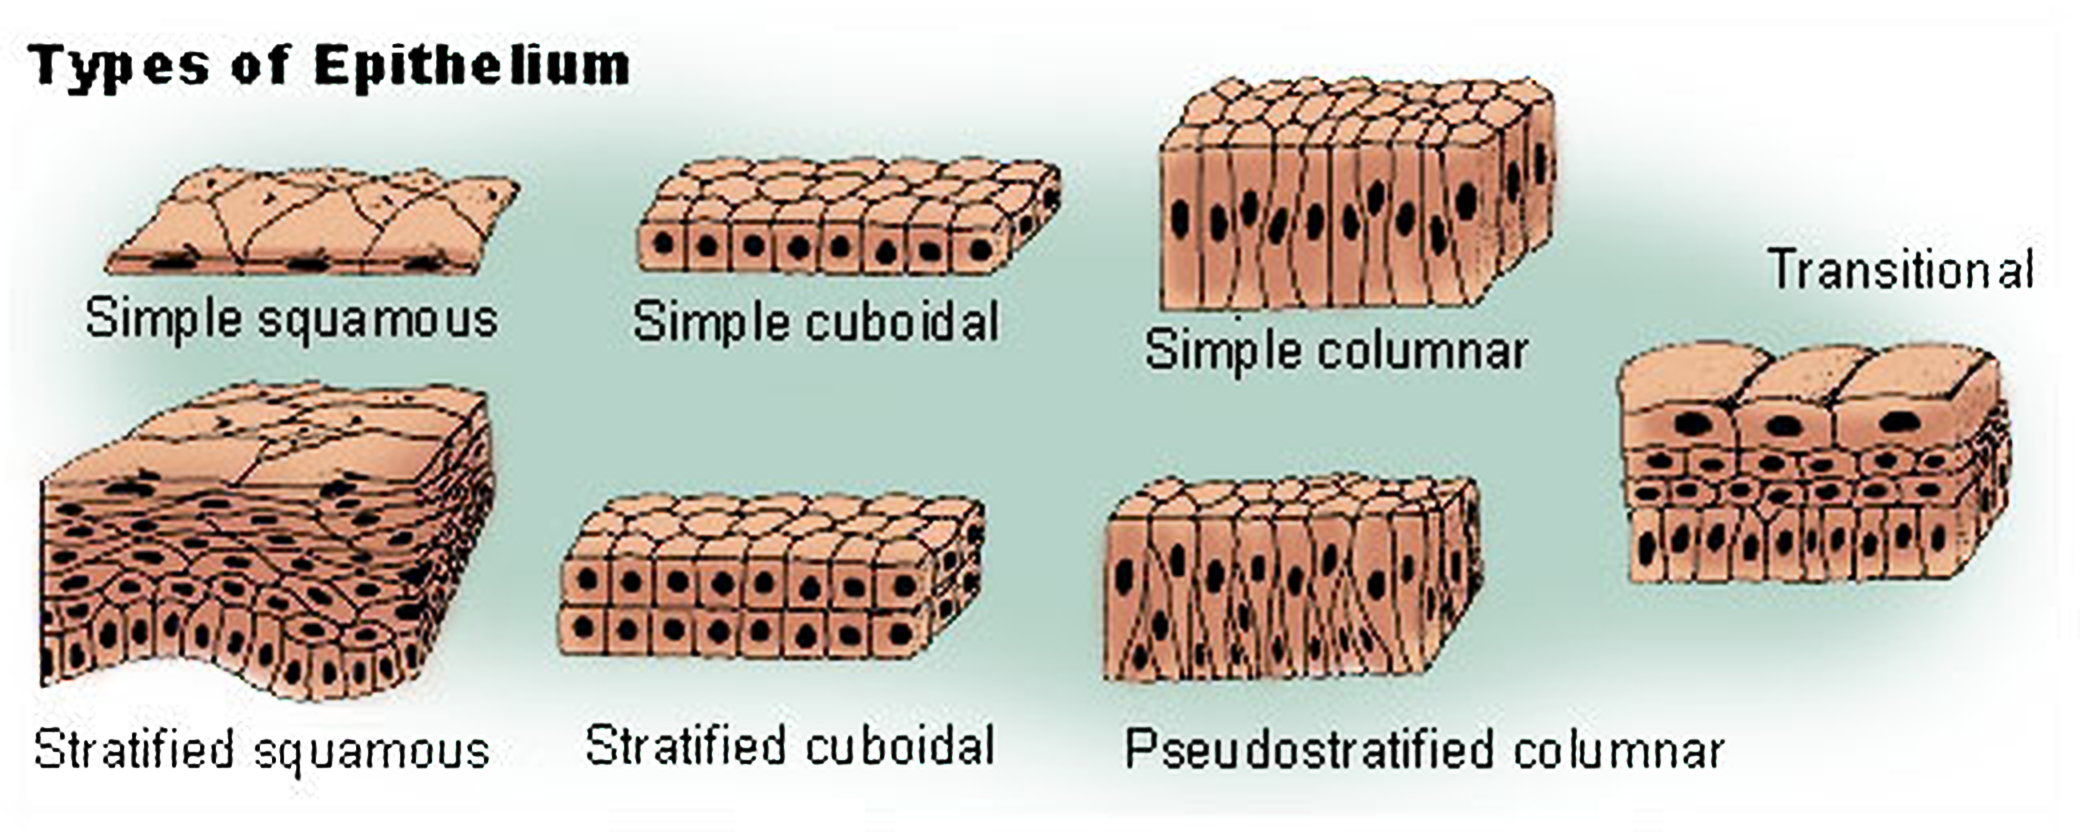
\includegraphics[width=\textwidth]{../diagrams/output.png}
\caption{The Types of Epithelial Tissue}
\label{fig:types}
\end{figure}

Botanical epithelia are rather simple and homogeneous - a single layer of cells covering exposed surfaces. As Figure~\ref{fig:types} shows, however, there are many types of epithelial tissue in animals which vary in the number of layers they include, how the cells are shaped, and how tall the cells are. Each of these types of cells are found in a different region of the body where they perform a specific function.  For example, the simple squamous epithelium is no more than one layer of cells thick, and the cells are all very flat, much flatter than they are wide. These cells are therefore well suited to  allow diffussion across themselves. As such, simple squamous tissue is found in the walls of blood vessels, and in the alveoli in the lungs, where the diffusion of oxygen occurs. On the other hand, columnar cells are much taller than they are wide, and are thus well suited to absorption. These cells are found in the intestines where they absorb nutrients from passing food. Stratified squamous epithelia are several layers thick line the esophogas and mouth and serve to protect against abraision.

What all of these tissues have in common, however, is how amenable they are to computational modeling. The simplest case is that of simple epithelia, which typically have near-uniform height, and very little difference in appearance between their apical and basal faces. This means that the cells can easily be approximated by two dimensional meshes, since the top and bottom of the cells move in tandem and the surface where two cells touch can be approximated by a line. Slightly more difficult is the modeling of stratified tissue. In this case, the tissue develops in three dimensions, since underlying cells affect the cells on top of them. These cannot be modeled in two dimensions, but can be modeled by a solid composed of three dimensional polytopes. The theory behind these models is well developed, but the techincal details of implementing such a model has made it so that very exist, and are often quite limited \footnote{Even a leading epithelial tissue simulator, Chaste, still does not have stable 3D modeling capabilities}. 

To give you an idea of what current epithelial tissue simulators have produced, I am putting some images from recent papers.

\begin{figure}[h]
    \centering
    \begin{subfigure}[b]{0.4\textwidth}
		\centering
		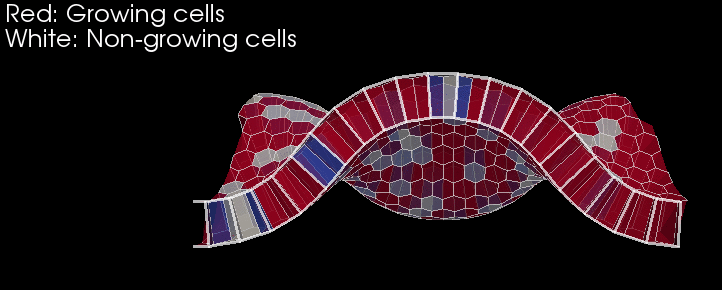
\includegraphics[width=\textwidth]{../diagrams/okuda1.png}
		\caption{Simple Squamous Tissue Bending in 3D\cite{Okuda1}}
		\label{fig:okuda1}
    \end{subfigure}
    \hfill
    \begin{subfigure}[b]{0.4\textwidth}
		\centering
		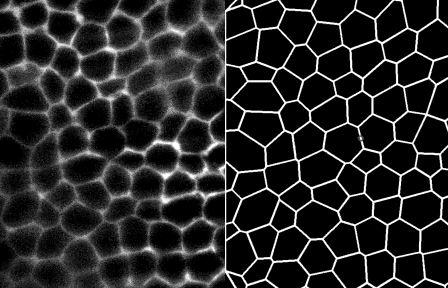
\includegraphics[width=\textwidth]{../diagrams/perfect.png}
		\caption{Comparison of Living Tissue and Simulation\cite{Yoshi}}
		\label{fig:yoshi}
    \end{subfigure}
    \hfill
    \begin{subfigure}[b]{0.4\textwidth}
        \centering
        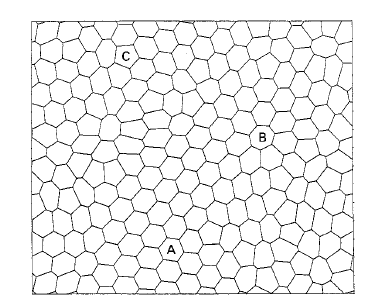
\includegraphics[width=\textwidth]{../diagrams/HondaResult.png}
        \caption{Equilibrium Mesh\cite{HondaNagai}}
        \label{fig:Honda}
    \end{subfigure}
    \hfill
    \begin{subfigure}[b]{0.4\textwidth}
        \centering
        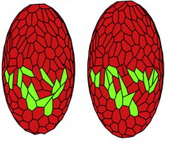
\includegraphics[width=\textwidth]{../diagrams/mirim.png}
        \caption{Equilibrium Mesh on a 3d Surface \cite{Vertex Models}}
        \label{fig:mirim}
    \end{subfigure}
    \caption{Some existing models of epithelial tissue.}
    \label{fig:four graphs}
\end{figure}


So, the question still remains: ``Why Study Epithelial Tissue?". The study of biological tissues has intrinsic value, much as mapping constellations or studying the properties of natural numbers. Beyond its inherent worth, current research in epithelial tissue is producing great results in the field of epithelial tissue  morphogenisis and diversifictation as well as wound healing. The Honda-Nagai model which we will discuss in great detail in this paper successfully reproduced the dynamics of the healing of wounds to cats' corneas\cite{Wound Healing}. This model has also been able to reproduce all of the essential dynamics of epithelial tissue \cite{HondaNagai}. So, in conclusion, we \emph{should} be modeling epithelial tissue computationally because it is easy to do, effective, an the community is currently very active and passionate about the field. 